%%%%%%%%%%%%%%%%%%%%%%%%%%%%%%%%%%%%%%%%%%%%%%%%%%%%%%%%%%%%%%%%%%%%%%%%%%
%
% 	Template for seminar reports
%
%%%%%%%%%%%%%%%%%%%%%%%%%%%%%%%%%%%%%%%%%%%%%%%%%%%%%%%%%%%%%%%%%%%%%%%%%%

%%%%%%%%%%%%%%%%%%%%%%%%%%%%%%%%%%%%%%%%%%%%%%%%%%%%%%%%%%%%%%%%%%%%%%%%%%
% 	Include layout and macros
%%%%%%%%%%%%%%%%%%%%%%%%%%%%%%%%%%%%%%%%%%%%%%%%%%%%%%%%%%%%%%%%%%%%%%%%%%
%% This LaTeX template is based on the following example file included in the ieeetran
%% package:
%% bare_conf.tex 
%% V1.2
%% 2002/11/18
%% by Michael Shell 
%% mshell@ece.gatech.edu
%% (requires IEEEtran.cls version 1.6b or later) with an IEEE conference paper.


% Note that the a4paper option is mainly intended so that authors in
% countries using A4 can easily print to A4 and see how their papers will
% look in print. Authors are encouraged to use U.S. letter paper when 
% submitting to IEEE. Use the testflow package mentioned above to verify
% correct handling of both paper sizes by the author's LaTeX system.
%
% Also note that the "draftcls" or "draftclsnofoot", not "draft", option
% should be used if it is desired that the figures are to be displayed in
% draft mode.
%
% This paper can be formatted using the peerreviewca
% (instead of conference) mode.
\documentclass[conference, a4paper]{bibliography/IEEEtran-modified}
% If the IEEEtran.cls has not been installed into the LaTeX system files, 
% manually specify the path to it:
% \documentclass[conference]{../sty/IEEEtran} 

\IEEEoverridecommandlockouts

% some very useful LaTeX packages include:

\usepackage{cite}       % Written by Donald Arseneau
                        % V1.6 and later of IEEEtran pre-defines the format
                        % of the cite.sty package \cite{} output to follow
                        % that of IEEE. Loading the cite package will
                        % result in citation numbers being automatically
                        % sorted and properly "ranged". i.e.,
                        % [1], [9], [2], [7], [5], [6]
                        % (without using cite.sty)
                        % will become:
                        % [1], [2], [5]--[7], [9] (using cite.sty)
                        % cite.sty's \cite will automatically add leading
                        % space, if needed. Use cite.sty's noadjust option
                        % (cite.sty V3.8 and later) if you want to turn this
                        % off. cite.sty is already installed on most LaTeX
                        % systems. The latest version can be obtained at:
                        % http://www.ctan.org/tex-archive/macros/latex/contrib/supported/cite/

%\usepackage{graphicx}  % Written by David Carlisle and Sebastian Rahtz
                        % Required if you want graphics, photos, etc.
                        % graphicx.sty is already installed on most LaTeX
                        % systems. The latest version and documentation can
                        % be obtained at:
                        % http://www.ctan.org/tex-archive/macros/latex/required/graphics/
                        % Another good source of documentation is "Using
                        % Imported Graphics in LaTeX2e" by Keith Reckdahl
                        % which can be found as esplatex.ps and epslatex.pdf
                        % at: http://www.ctan.org/tex-archive/info/
% NOTE: for dual use with latex and pdflatex, instead load graphicx like:
\ifx\pdfoutput\undefined
	\usepackage{graphicx}
\else
	\usepackage[pdftex]{graphicx}
\fi

% However, be warned that pdflatex will require graphics to be in PDF
% (not EPS) format and will preclude the use of PostScript based LaTeX
% packages such as psfrag.sty and pstricks.sty. IEEE conferences typically
% allow PDF graphics (and hence pdfLaTeX). However, IEEE journals do not
% (yet) allow image formats other than EPS or TIFF. Therefore, authors of
% journal papers should use traditional LaTeX with EPS graphics.
%
% The path(s) to the graphics files can also be declared: e.g.,
% \graphicspath{{../eps/}{../ps/}}
% if the graphics files are not located in the same directory as the
% .tex file. This can be done in each branch of the conditional above
% (after graphicx is loaded) to handle the EPS and PDF cases separately.
% In this way, full path information will not have to be specified in
% each \includegraphics command.
%
% Note that, when switching from latex to pdflatex and vice-versa, the new
% compiler will have to be run twice to clear some warnings.
\graphicspath{{figures/}}


%\usepackage{psfrag}    % Written by Craig Barratt, Michael C. Grant,
                        % and David Carlisle
                        % This package allows you to substitute LaTeX
                        % commands for text in imported EPS graphic files.
                        % In this way, LaTeX symbols can be placed into
                        % graphics that have been generated by other
                        % applications. You must use latex->dvips->ps2pdf
                        % workflow (not direct pdf output from pdflatex) if
                        % you wish to use this capability because it works
                        % via some PostScript tricks. Alternatively, the
                        % graphics could be processed as separate files via
                        % psfrag and dvips, then converted to PDF for
                        % inclusion in the main file which uses pdflatex.
                        % Docs are in "The PSfrag System" by Michael C. Grant
                        % and David Carlisle. There is also some information 
                        % about using psfrag in "Using Imported Graphics in
                        % LaTeX2e" by Keith Reckdahl which documents the
                        % graphicx package (see above). The psfrag package
                        % and documentation can be obtained at:
                        % http://www.ctan.org/tex-archive/macros/latex/contrib/supported/psfrag/

%\usepackage{subfigure} % Written by Steven Douglas Cochran
                        % This package makes it easy to put subfigures
                        % in your figures. i.e., "figure 1a and 1b"
                        % Docs are in "Using Imported Graphics in LaTeX2e"
                        % by Keith Reckdahl which also documents the graphicx
                        % package (see above). subfigure.sty is already
                        % installed on most LaTeX systems. The latest version
                        % and documentation can be obtained at:
                        % http://www.ctan.org/tex-archive/macros/latex/contrib/supported/subfigure/

%\usepackage{url}       % Written by Donald Arseneau
                        % Provides better support for handling and breaking
                        % URLs. url.sty is already installed on most LaTeX
                        % systems. The latest version can be obtained at:
                        % http://www.ctan.org/tex-archive/macros/latex/contrib/other/misc/
                        % Read the url.sty source comments for usage information.

%\usepackage{stfloats}  % Written by Sigitas Tolusis
                        % Gives LaTeX2e the ability to do double column
                        % floats at the bottom of the page as well as the top.
                        % (e.g., "\begin{figure*}[!b]" is not normally
                        % possible in LaTeX2e). This is an invasive package
                        % which rewrites many portions of the LaTeX2e output
                        % routines. It may not work with other packages that
                        % modify the LaTeX2e output routine and/or with other
                        % versions of LaTeX. The latest version and
                        % documentation can be obtained at:
                        % http://www.ctan.org/tex-archive/macros/latex/contrib/supported/sttools/
                        % Documentation is contained in the stfloats.sty
                        % comments as well as in the presfull.pdf file.
                        % Do not use the stfloats baselinefloat ability as
                        % IEEE does not allow \baselineskip to stretch.
                        % Authors submitting work to the IEEE should note
                        % that IEEE rarely uses double column equations and
                        % that authors should try to avoid such use.
                        % Do not be tempted to use the cuted.sty or
                        % midfloat.sty package (by the same author) as IEEE
                        % does not format its papers in such ways.

\usepackage{amsmath}    % From the American Mathematical Society
                        % A popular package that provides many helpful commands
                        % for dealing with mathematics. Note that the AMSmath
                        % package sets \interdisplaylinepenalty to 10000 thus
                        % preventing page breaks from occurring within multiline
                        % equations. Use:
\interdisplaylinepenalty=2500
                        % after loading amsmath to restore such page breaks
                        % as IEEEtran.cls normally does. amsmath.sty is already
                        % installed on most LaTeX systems. The latest version
                        % and documentation can be obtained at:
                        % http://www.ctan.org/tex-archive/macros/latex/required/amslatex/math/
%\usepackage[T1]{fontenc}
\usepackage[utf8]{inputenc}
%\usepackage[latin1]{inputenc}   % für Umlaute 
\renewcommand{\keywordname}{Keywords}

% Other popular packages for formatting tables and equations include:

%\usepackage{array}
% Frank Mittelbach's and David Carlisle's array.sty which improves the
% LaTeX2e array and tabular environments to provide better appearances and
% additional user controls. array.sty is already installed on most systems.
% The latest version and documentation can be obtained at:
% http://www.ctan.org/tex-archive/macros/latex/required/tools/

% Mark Wooding's extremely powerful MDW tools, especially mdwmath.sty and
% mdwtab.sty which are used to format equations and tables, respectively.
% The MDWtools set is already installed on most LaTeX systems. The lastest
% version and documentation is available at:
% http://www.ctan.org/tex-archive/macros/latex/contrib/supported/mdwtools/


% V1.6 of IEEEtran contains the IEEEeqnarray family of commands that can
% be used to generate multiline equations as well as matrices, tables, etc.


% Also of notable interest:

% Scott Pakin's eqparbox package for creating (automatically sized) equal
% width boxes. Available:
% http://www.ctan.org/tex-archive/macros/latex/contrib/supported/eqparbox/



% Notes on hyperref:
% IEEEtran.cls attempts to be compliant with the hyperref package, written
% by Heiko Oberdiek and Sebastian Rahtz, which provides hyperlinks within
% a document as well as an index for PDF files (produced via pdflatex).
% However, it is a tad difficult to properly interface LaTeX classes and
% packages with this (necessarily) complex and invasive package. It is
% recommended that hyperref not be used for work that is to be submitted
% to the IEEE. Users who wish to use hyperref *must* ensure that their
% hyperref version is 6.72u or later *and* IEEEtran.cls is version 1.6b 
% or later. The latest version of hyperref can be obtained at:
%
% http://www.ctan.org/tex-archive/macros/latex/contrib/supported/hyperref/
%
% Also, be aware that cite.sty (as of version 3.9, 11/2001) and hyperref.sty
% (as of version 6.72t, 2002/07/25) do not work optimally together.
% To mediate the differences between these two packages, IEEEtran.cls, as
% of v1.6b, predefines a command that fools hyperref into thinking that
% the natbib package is being used - causing it not to modify the existing
% citation commands, and allowing cite.sty to operate as normal. However,
% as a result, citation numbers will not be hyperlinked. Another side effect
% of this approach is that the natbib.sty package will not properly load
% under IEEEtran.cls. However, current versions of natbib are not capable
% of compressing and sorting citation numbers in IEEE's style - so this
% should not be an issue. If, for some strange reason, the user wants to
% load natbib.sty under IEEEtran.cls, the following code must be placed
% before natbib.sty can be loaded:
%
% \makeatletter
% \let\NAT@parse\undefined
% \makeatother
%
% Hyperref should be loaded differently depending on whether pdflatex
% or traditional latex is being used:
%
%\ifx\pdfoutput\undefined
%\usepackage[hypertex]{hyperref}
%\else
%\usepackage[pdftex,hypertexnames=false]{hyperref}
%\fi
%
% Pdflatex produces superior hyperref results and is the recommended
% compiler for such use.

% *** Do not adjust lengths that control margins, column widths, etc. ***
% *** Do not use packages that alter fonts (such as pslatex).         ***
% There should be no need to do such things with IEEEtran.cls V1.6 and later.
%%% This LaTeX template is based on the following example file included in the ieeetran
%% package:
%% bare_conf.tex 
%% V1.2
%% 2002/11/18
%% by Michael Shell
%% mshell@ece.gatech.edu
%% (requires IEEEtran.cls version 1.6b or later) with an IEEE conference paper.


% Note that the a4paper option is mainly intended so that authors in
% countries using A4 can easily print to A4 and see how their papers will
% look in print. Authors are encouraged to use U.S. letter paper when 
% submitting to IEEE. Use the testflow package mentioned above to verify
% correct handling of both paper sizes by the author's LaTeX system.
%
% Also note that the "draftcls" or "draftclsnofoot", not "draft", option
% should be used if it is desired that the figures are to be displayed in
% draft mode.
%
% This paper can be formatted using the peerreviewca
% (instead of conference) mode.
\documentclass[conference, a4paper]{IEEEtran-modified}
% If the IEEEtran.cls has not been installed into the LaTeX system files, 
% manually specify the path to it:
% \documentclass[conference]{../sty/IEEEtran} 

\IEEEoverridecommandlockouts

% some very useful LaTeX packages include:

\usepackage{cite}       % Written by Donald Arseneau
                        % V1.6 and later of IEEEtran pre-defines the format
                        % of the cite.sty package \cite{} output to follow
                        % that of IEEE. Loading the cite package will
                        % result in citation numbers being automatically
                        % sorted and properly "ranged". i.e.,
                        % [1], [9], [2], [7], [5], [6]
                        % (without using cite.sty)
                        % will become:
                        % [1], [2], [5]--[7], [9] (using cite.sty)
                        % cite.sty's \cite will automatically add leading
                        % space, if needed. Use cite.sty's noadjust option
                        % (cite.sty V3.8 and later) if you want to turn this
                        % off. cite.sty is already installed on most LaTeX
                        % systems. The latest version can be obtained at:
                        % http://www.ctan.org/tex-archive/macros/latex/contrib/supported/cite/

%\usepackage{graphicx}  % Written by David Carlisle and Sebastian Rahtz
                        % Required if you want graphics, photos, etc.
                        % graphicx.sty is already installed on most LaTeX
                        % systems. The latest version and documentation can
                        % be obtained at:
                        % http://www.ctan.org/tex-archive/macros/latex/required/graphics/
                        % Another good source of documentation is "Using
                        % Imported Graphics in LaTeX2e" by Keith Reckdahl
                        % which can be found as esplatex.ps and epslatex.pdf
                        % at: http://www.ctan.org/tex-archive/info/
% NOTE: for dual use with latex and pdflatex, instead load graphicx like:
\ifx\pdfoutput\undefined
	\usepackage{graphicx}
\else
	\usepackage[pdftex]{graphicx}
\fi

% However, be warned that pdflatex will require graphics to be in PDF
% (not EPS) format and will preclude the use of PostScript based LaTeX
% packages such as psfrag.sty and pstricks.sty. IEEE conferences typically
% allow PDF graphics (and hence pdfLaTeX). However, IEEE journals do not
% (yet) allow image formats other than EPS or TIFF. Therefore, authors of
% journal papers should use traditional LaTeX with EPS graphics.
%
% The path(s) to the graphics files can also be declared: e.g.,
% \graphicspath{{../eps/}{../ps/}}
% if the graphics files are not located in the same directory as the
% .tex file. This can be done in each branch of the conditional above
% (after graphicx is loaded) to handle the EPS and PDF cases separately.
% In this way, full path information will not have to be specified in
% each \includegraphics command.
%
% Note that, when switching from latex to pdflatex and vice-versa, the new
% compiler will have to be run twice to clear some warnings.
\graphicspath{{figures/}}


%\usepackage{psfrag}    % Written by Craig Barratt, Michael C. Grant,
                        % and David Carlisle
                        % This package allows you to substitute LaTeX
                        % commands for text in imported EPS graphic files.
                        % In this way, LaTeX symbols can be placed into
                        % graphics that have been generated by other
                        % applications. You must use latex->dvips->ps2pdf
                        % workflow (not direct pdf output from pdflatex) if
                        % you wish to use this capability because it works
                        % via some PostScript tricks. Alternatively, the
                        % graphics could be processed as separate files via
                        % psfrag and dvips, then converted to PDF for
                        % inclusion in the main file which uses pdflatex.
                        % Docs are in "The PSfrag System" by Michael C. Grant
                        % and David Carlisle. There is also some information 
                        % about using psfrag in "Using Imported Graphics in
                        % LaTeX2e" by Keith Reckdahl which documents the
                        % graphicx package (see above). The psfrag package
                        % and documentation can be obtained at:
                        % http://www.ctan.org/tex-archive/macros/latex/contrib/supported/psfrag/

%\usepackage{subfigure} % Written by Steven Douglas Cochran
                        % This package makes it easy to put subfigures
                        % in your figures. i.e., "figure 1a and 1b"
                        % Docs are in "Using Imported Graphics in LaTeX2e"
                        % by Keith Reckdahl which also documents the graphicx
                        % package (see above). subfigure.sty is already
                        % installed on most LaTeX systems. The latest version
                        % and documentation can be obtained at:
                        % http://www.ctan.org/tex-archive/macros/latex/contrib/supported/subfigure/

%\usepackage{url}       % Written by Donald Arseneau
                        % Provides better support for handling and breaking
                        % URLs. url.sty is already installed on most LaTeX
                        % systems. The latest version can be obtained at:
                        % http://www.ctan.org/tex-archive/macros/latex/contrib/other/misc/
                        % Read the url.sty source comments for usage information.

%\usepackage{stfloats}  % Written by Sigitas Tolusis
                        % Gives LaTeX2e the ability to do double column
                        % floats at the bottom of the page as well as the top.
                        % (e.g., "\begin{figure*}[!b]" is not normally
                        % possible in LaTeX2e). This is an invasive package
                        % which rewrites many portions of the LaTeX2e output
                        % routines. It may not work with other packages that
                        % modify the LaTeX2e output routine and/or with other
                        % versions of LaTeX. The latest version and
                        % documentation can be obtained at:
                        % http://www.ctan.org/tex-archive/macros/latex/contrib/supported/sttools/
                        % Documentation is contained in the stfloats.sty
                        % comments as well as in the presfull.pdf file.
                        % Do not use the stfloats baselinefloat ability as
                        % IEEE does not allow \baselineskip to stretch.
                        % Authors submitting work to the IEEE should note
                        % that IEEE rarely uses double column equations and
                        % that authors should try to avoid such use.
                        % Do not be tempted to use the cuted.sty or
                        % midfloat.sty package (by the same author) as IEEE
                        % does not format its papers in such ways.

\usepackage{amsmath}    % From the American Mathematical Society
                        % A popular package that provides many helpful commands
                        % for dealing with mathematics. Note that the AMSmath
                        % package sets \interdisplaylinepenalty to 10000 thus
                        % preventing page breaks from occurring within multiline
                        % equations. Use:
\interdisplaylinepenalty=2500
                        % after loading amsmath to restore such page breaks
                        % as IEEEtran.cls normally does. amsmath.sty is already
                        % installed on most LaTeX systems. The latest version
                        % and documentation can be obtained at:
                        % http://www.ctan.org/tex-archive/macros/latex/required/amslatex/math/
%\usepackage[T1]{fontenc}
\usepackage[utf8]{inputenc}
%\usepackage[latin1]{inputenc}   % für Umlaute 
\renewcommand{\keywordname}{Keywords}

% Other popular packages for formatting tables and equations include:

%\usepackage{array}
% Frank Mittelbach's and David Carlisle's array.sty which improves the
% LaTeX2e array and tabular environments to provide better appearances and
% additional user controls. array.sty is already installed on most systems.
% The latest version and documentation can be obtained at:
% http://www.ctan.org/tex-archive/macros/latex/required/tools/

% Mark Wooding's extremely powerful MDW tools, especially mdwmath.sty and
% mdwtab.sty which are used to format equations and tables, respectively.
% The MDWtools set is already installed on most LaTeX systems. The lastest
% version and documentation is available at:
% http://www.ctan.org/tex-archive/macros/latex/contrib/supported/mdwtools/


% V1.6 of IEEEtran contains the IEEEeqnarray family of commands that can
% be used to generate multiline equations as well as matrices, tables, etc.


% Also of notable interest:

% Scott Pakin's eqparbox package for creating (automatically sized) equal
% width boxes. Available:
% http://www.ctan.org/tex-archive/macros/latex/contrib/supported/eqparbox/



% Notes on hyperref:
% IEEEtran.cls attempts to be compliant with the hyperref package, written
% by Heiko Oberdiek and Sebastian Rahtz, which provides hyperlinks within
% a document as well as an index for PDF files (produced via pdflatex).
% However, it is a tad difficult to properly interface LaTeX classes and
% packages with this (necessarily) complex and invasive package. It is
% recommended that hyperref not be used for work that is to be submitted
% to the IEEE. Users who wish to use hyperref *must* ensure that their
% hyperref version is 6.72u or later *and* IEEEtran.cls is version 1.6b 
% or later. The latest version of hyperref can be obtained at:
%
% http://www.ctan.org/tex-archive/macros/latex/contrib/supported/hyperref/
%
% Also, be aware that cite.sty (as of version 3.9, 11/2001) and hyperref.sty
% (as of version 6.72t, 2002/07/25) do not work optimally together.
% To mediate the differences between these two packages, IEEEtran.cls, as
% of v1.6b, predefines a command that fools hyperref into thinking that
% the natbib package is being used - causing it not to modify the existing
% citation commands, and allowing cite.sty to operate as normal. However,
% as a result, citation numbers will not be hyperlinked. Another side effect
% of this approach is that the natbib.sty package will not properly load
% under IEEEtran.cls. However, current versions of natbib are not capable
% of compressing and sorting citation numbers in IEEE's style - so this
% should not be an issue. If, for some strange reason, the user wants to
% load natbib.sty under IEEEtran.cls, the following code must be placed
% before natbib.sty can be loaded:
%
% \makeatletter
% \let\NAT@parse\undefined
% \makeatother
%
% Hyperref should be loaded differently depending on whether pdflatex
% or traditional latex is being used:
%
%\ifx\pdfoutput\undefined
%\usepackage[hypertex]{hyperref}
%\else
%\usepackage[pdftex,hypertexnames=false]{hyperref}
%\fi
%
% Pdflatex produces superior hyperref results and is the recommended
% compiler for such use.

% *** Do not adjust lengths that control margins, column widths, etc. ***
% *** Do not use packages that alter fonts (such as pslatex).         ***
% There should be no need to do such things with IEEEtran.cls V1.6 and later.
%
%%%%%%%%%%%%%%%%%%%%%%%%%%%%%%%%%%%%%%%%%%%%%%%%%%%%%%%%%%%%%%%%%%%%%%%%%%
% 	Anpassung an deutsche Texte
%%%%%%%%%%%%%%%%%%%%%%%%%%%%%%%%%%%%%%%%%%%%%%%%%%%%%%%%%%%%%%%%%%%%%%%%%%

\usepackage{ngerman}
\usepackage[latin1]{inputenc}   % für Umlaute 

%\renewcommand{\abstractname}{Kurzfassung}      % statt Zusammenfassung, wie es ngerman definiert
%\renewcommand{\keywordname}{Schlüsselworte}
%\renewcommand{\figurename}{Abb.}


 %uncomment in case you write in German

%%%%%%%%%%%%%%%%%%%%%%%%%%%%%%%%%%%%%%%%%%%%%%%%%%%%%%%%%%%%%%%%%%%%%%%%%%
% 	Page numbering (not on first page)
%%%%%%%%%%%%%%%%%%%%%%%%%%%%%%%%%%%%%%%%%%%%%%%%%%%%%%%%%%%%%%%%%%%%%%%%%%
\pagestyle{empty}

%%%%%%%%%%%%%%%%%%%%%%%%%%%%%%%%%%%%%%%%%%%%%%%%%%%%%%%%%%%%%%%%%%%%%%%%%%
% 	Correct bad hyphenation here
%%%%%%%%%%%%%%%%%%%%%%%%%%%%%%%%%%%%%%%%%%%%%%%%%%%%%%%%%%%%%%%%%%%%%%%%%%

\hyphenation{}

%%%%%%%%%%%%%%%%%%%%%%%%%%%%%%%%%%%%%%%%%%%%%%%%%%%%%%%%%%%%%%%%%%%%%%%%%%
% 	Begin of the document
%%%%%%%%%%%%%%%%%%%%%%%%%%%%%%%%%%%%%%%%%%%%%%%%%%%%%%%%%%%%%%%%%%%%%%%%%%

\begin{document}

%%%%%%%%%%%%%%%%%%%%%%%%%%%%%%%%%%%%%%%%%%%%%%%%%%%%%%%%%%%%%%%%%%%%%%%%%%
% 	Paper title
%%%%%%%%%%%%%%%%%%%%%%%%%%%%%%%%%%%%%%%%%%%%%%%%%%%%%%%%%%%%%%%%%%%%%%%%%%

\title{Title of the Seminar Paper}

%%%%%%%%%%%%%%%%%%%%%%%%%%%%%%%%%%%%%%%%%%%%%%%%%%%%%%%%%%%%%%%%%%%%%%%%%%
% 	Author names and affiliations 
%		-	multiple columns for up to three different affilitations are separated 
%			by \and
%		- for over three affiliations, refer to ieeetran howto
%%%%%%%%%%%%%%%%%%%%%%%%%%%%%%%%%%%%%%%%%%%%%%%%%%%%%%%%%%%%%%%%%%%%%%%%%%

\author{
\authorblockN{Julien Schulz}
\authorblockA{Department of Informatics\\Technische Universität München\\
Email: julien.schulz@tum.de} 
\and
\authorblockN{Michael Cegielka}
\authorblockA{Department of Informatics\\Universität Bremen\\
Email: mi\_ce@uni-bremen.de} 
\and
\authorblockN{Leonhard Zirus}
\authorblockA{Department of Informatics\\Technische Universität München\\
Email: leonhard.zirus@tum.de} 
%\and
%\authorblockN{}
%\authorblockA{}
}

%%%%%%%%%%%%%%%%%%%%%%%%%%%%%%%%%%%%%%%%%%%%%%%%%%%%%%%%%%%%%%%%%%%%%%%%%%
% 	Special paper note (appears between title and authors) 
%%%%%%%%%%%%%%%%%%%%%%%%%%%%%%%%%%%%%%%%%%%%%%%%%%%%%%%%%%%%%%%%%%%%%%%%%%

\specialpapernotice{Neural Network Learning}

%%%%%%%%%%%%%%%%%%%%%%%%%%%%%%%%%%%%%%%%%%%%%%%%%%%%%%%%%%%%%%%%%%%%%%%%%%
% 	Make title area 
%%%%%%%%%%%%%%%%%%%%%%%%%%%%%%%%%%%%%%%%%%%%%%%%%%%%%%%%%%%%%%%%%%%%%%%%%%

\maketitle

%%%%%%%%%%%%%%%%%%%%%%%%%%%%%%%%%%%%%%%%%%%%%%%%%%%%%%%%%%%%%%%%%%%%%%%%%%
% 	For page number on first page
%%%%%%%%%%%%%%%%%%%%%%%%%%%%%%%%%%%%%%%%%%%%%%%%%%%%%%%%%%%%%%%%%%%%%%%%%%

%\thispagestyle{plain}

%%%%%%%%%%%%%%%%%%%%%%%%%%%%%%%%%%%%%%%%%%%%%%%%%%%%%%%%%%%%%%%%%%%%%%%%%%
% 	Abstract 
%%%%%%%%%%%%%%%%%%%%%%%%%%%%%%%%%%%%%%%%%%%%%%%%%%%%%%%%%%%%%%%%%%%%%%%%%%


\begin{abstract}

This paper documents the entire process of creating a machine learning model,
that is capable to determine, whether a person is wearing a mask or not, on
basis of an image of that person. The project includes the creation of an
annotation software used to edit and pre-process the used dataset as well as the
implementation, training and testing of the model itself.

\end{abstract}


%%%%%%%%%%%%%%%%%%%%%%%%%%%%%%%%%%%%%%%%%%%%%%%%%%%%%%%%%%%%%%%%%%%%%%%%%%
% 	Keywords 
%%%%%%%%%%%%%%%%%%%%%%%%%%%%%%%%%%%%%%%%%%%%%%%%%%%%%%%%%%%%%%%%%%%%%%%%%%

\begin{keywords}
Machine Learning, 
\end{keywords}


%%%%%%%%%%%%%%%%%%%%%%%%%%%%%%%%%%%%%%%%%%%%%%%%%%%%%%%%%%%%%%%%%%%%%%%%%%
% 	Sections, Subsections,...
%%%%%%%%%%%%%%%%%%%%%%%%%%%%%%%%%%%%%%%%%%%%%%%%%%%%%%%%%%%%%%%%%%%%%%%%%%

\section{Introduction}

With software infusing more and more of our daily lives, software developers are
trying to keep up with the rising expectations of end-users. With IoT in the
rise, we collect more data in a single day, than we could have ever imagined and
have digital interfaces to nearly all parts of our lives. 


Software development has grown to a point, where we have a giant base of great
algorithms, that enable us to solve many problems quickly and efficiently. In
todays software development it often comes down to having an idea and
implementing it on the basis of these existing algorithms. Still there is a
limit to what they can do and it is often reached at tasks that seam pretty
simple to us humans. Algorithms are great in using big amounts of data,
accumulating it to models and trends, showing it in smart graphs and in general
making it visual and easier to analyse and interpret. Still the final
interpretation is a skill where humans are unmatched in. 


The following paper follows the entire process of creating a so called
"artificial intelligence" that is able to take an image, grabbed from a file or
a video and determine, if showing a person, which kind of mask this person is
wearing or whether he/she is wearing any at all. First the project and its goals
will be layed out in detail with a short introduction of each team member and
their role in this project. This is followed by a description of the used
dataset and how it was created. Then there will be an outline of the process
including used methodologies and encountered difficulties and finally a
summarization of the obtained results and their interpretation. 


\section{Project - Description}

This project was conducted in context of a university course at Université Côte
d'Azur in Nice, France. The main goal of the project was a first experimentation
with the concept of machine learning with neural networks. It's purpose was to
gain a deeper understanding of what influences the decisions of such a model and
using the gained knowledge to create a simple, but fully functioning
face-mask-detector.
\newline
The project was split into two parts, the data collection and preparation and
the machine learning (ML) model creation and training. In the following both
parts will be outlined with a introduction of the team members and their roles
in both parts.

\subsection{Part I - Data Collection and Preparation}

The data collection is already a big part of the project, as there are a lot of
things that can go wrong here. The data is the main influence of the
final model and the decisions it makes. A ML model does not differ a lot from humans
in this context, as both can only act on their own experiences. Therefore
making sure the data is chosen in conjunction with the final goals is essential.
As the scale of this project is fairly small and its purpose is a first
experimentation with the concept, it was sufficient to expect the model to
recognize the three members of this project.
\newline
The collected data will most likely not be in a format, that is easily readable
for our model. The next step therefore needs to manually interpret the data,
label it for the model and standardize it. The level of the data preprocessing
again is determined by the goal one wants to achieve. In the scale of this
project, our preprocessing will go as far as already identifying the face on the
image, cutting it to a good fitting square and giving it a label according to
its context.
\newline
To achieve all that in a streamlined, standardized and user friendly way, the
development of an image annotation software was necessary. In addition to the
manual annotation there are some automation tricks that can be used to help with
easily classifiable data. 

\subsection{Part II - Machine Learning Model}

This of course is the center of the project. Setting up and compiling a ML
model, capable of, given an image of a face, determining whether the
person shown is wearing a mask and what kind if yes.
\newline
As mentioned before, the goal was limited to being able to detect masks on the
faces of the team members of this project, as we would have needed a much larger
and more diverse dataset to achieve reliable results with all other faces. Still
the hope is, that the model will be able to generalize and extend to more, 
mostly similar faces. This will probably include white, western
men. Difficulties might occur with people of color, with different facial structures or women.

\subsection{Team Members and Roles}

The team consists of three members, Michael Cegielka, Julien Schulz and Leonhard
Zirus. The roles in this project where distributed equally in a way where
everyone was still involved in every part of it. 
\newline
In the first part of the project, Leonhard took charge of the annotation
software, being responsible for the organization and collaboration. He created
the framework and interfaces. Julien as our ML expert was responsible for making
sure that the software was usable in the second part of the project and created
a streamlined process for the creation of the dataset, augmentation and later
labeling. Micheal was mainly in charge of the UI (User Interface) and UE (User
Experience) of the annotation software. 
\newline
The coding of the first part was mainly done by Leonhard, who delegated jobs to the others.
The code for the second part was mainly developed by Julien, with the help of his teammates
and Leonhard, who linked the interfaces.
The paper was written by Leonhard, who was in direct communication with the expert of
each chapter. It was then corrected and slightly adjusted by all team members.

\section{Dataset}

The used dataset was created by taking pictures of our team members wearing
different kinds of masks. For the ML model to use the images they need to be
preprocessed and labeled to enable the learning process.

\subsection{Image Creation}

The images taken will influence greatly what kind of images the model will later
be able to recognize. This means, that lighting, orientation of the face,
background, clothing or other kinds of patterns are very important to be aware
of when creating the pictures. 
\newline
Imagine a person choses to never wear a bonnet when walking inside, but because
of corona, that is exactly when he/she always wears a mask. As it is winter, the
opposite is true for being outside, he/she wears a bonnet, as it is cold, but no
mask, because it is outside and not required. Now using pictures from these
situations, the model might turn to identifying whether the person is wearing a
bonnet instead, as the dataset reflects such an implication. This is just one of
many examples, of unwilling implications that might turn up in a dataset.
\newline
In order to make sure to not have any such implications the images were tried to
create, using equal distributions of different backgrounds, with no lighting
differences correlating to the wearing or not wearing of a mask and different
clothing styles not related to the mask. The later one was limited to wearing a
bonnet or not.
\newline
The limitation of time and equipment will surely create a few problems with the
dataset. As an example, the creation started in the evening, which in turn
changed the lighting between changing to a different mask. As this problem
became aware, the fotoshoot was moved inside to at least have similar lighting
throughout all the pictures.
\newline
The improvements to the creation are countless, but would have all not been
justified by the dimension of this project. To create a proper one, the
diversity of the people, lighting, backgrounds, clothing, camera-lenses, etc.
would all have to be greatly increased. Also the number of images created is
still very small for the model to accurately recognize anyone, anywhere we put
them in front of the camera. In the end the created dataset should have
sufficient diversity to serve the purpose of this project.

\subsection{Scaling, Labeling and Formatting}

With the base for the dataset created, it is time to pre-process the images into
a format that can be used for the model. The final images should have a square
format with 240 x 240 pixels saved in a folder specifying it's label. There are
four labels: "no\_mask", "ffp2", "op\_mask" and "other\_mask". In this case
"other\_mask" will be different kinds of cloth-masks.
\newline
To limit the manual work as much as possible, the usage of the OpenCV
Haar-Cascade-Classifier, which is a pre-trained algorithm to detect faces on an
image. A short script enabled the automated loading of all images in a folder,
computation of present faces, cropping of the face in the image and saving it in
a new location. As the cascade classifier gives a whole lot of false positives,
it is important to got through the exported files and delete anything that can
not be used. To help figure out which image was already correctly processed,
there is a second small script comparing the processed images to the raw images
and copying all unprocessed ones to a new folder, ready to be manually
annotated. 
\newline
The labeling process of course can't be automated, as this would already be the
finished model. The processed images therefore have to be manually copied in
their respective folders.
\newline
The missing images, now have to be manually annotated, where finally the
image annotator comes to play. Using this software it is just a matter of going
through all remaining images, marking each face with a bounding box and labeling
it correctly. Afterwards the Annotator offers a crop and save function, that
takes care of cropping, scaling and correctly saving the images in the right
labeled folders.


\section{Implementation and Methodologies}

This project had two major implementations, the annotator and the ML model,
which will be detailed in this chapter. The following will explain used
methodologies and choices made in the implementation process as well as overcome
difficulties. 

\subsection{Image-Annotator}

The purpose of the image annotation software is to give an easy possibility of
labeling, rescaling, cropping and saving images in order to be used as dataset
by the ML model.
\newline
The software was completely written in python, an interpreted script language.
Still python has object oriented features, that where partly used in this
project. 
\newline
The program program is structured in a way, to have two different classes,
"Window" and "popupWindow" to take care of the UI part of the project. The rest
of the functionality is structured into script-like functions. This structuring
makes it easier to split the program into smaller tasks that can be distributed
and worked on individually. This is a methodology oriented at the MVC (Model
View Controller) software development pattern. The UI is here clearly separated
from the controlling instance, that handles the backend of user interaction as
well as the model, which is responsible for data storage and maintenance. As
this is a simple single instance application, of course a detailed
implementation was not necessary and the model and controller are somewhat mixed
and both just represented as the separate functions. Still it gives the
possibility of separating the implementation of the UI, the backend and the
storage system.
\newline
The UI is handled by the the tkinter python library, which gives a lot of basic
functionality to easily implement the frontend of the application. The UI of
this project was mainly focused on the menu bar on top in addition to a
right-click menu. This choice was made in order to keep the overall frame clean
and focused on the most important thing, the image.
\newline
The backend storage uses a python dictionary to at all time store all edits made
by the software. If need be, the entirety of the data can be saved to file using
the JSON format and loaded back from it as well. To keep the storage as
efficient as possible and maintain the possibility to easily change categories,
they are saved separately with a second array only linking the index of
the annotation to the index of a category. Listing 1 shows a reduced example of
stored annotations. There is a feature enabling the user to save every processed
resized image to a specified location. It was disabled as it turned out not to
be needed in this project. 

\begin{figure*}[t]
    \centering
    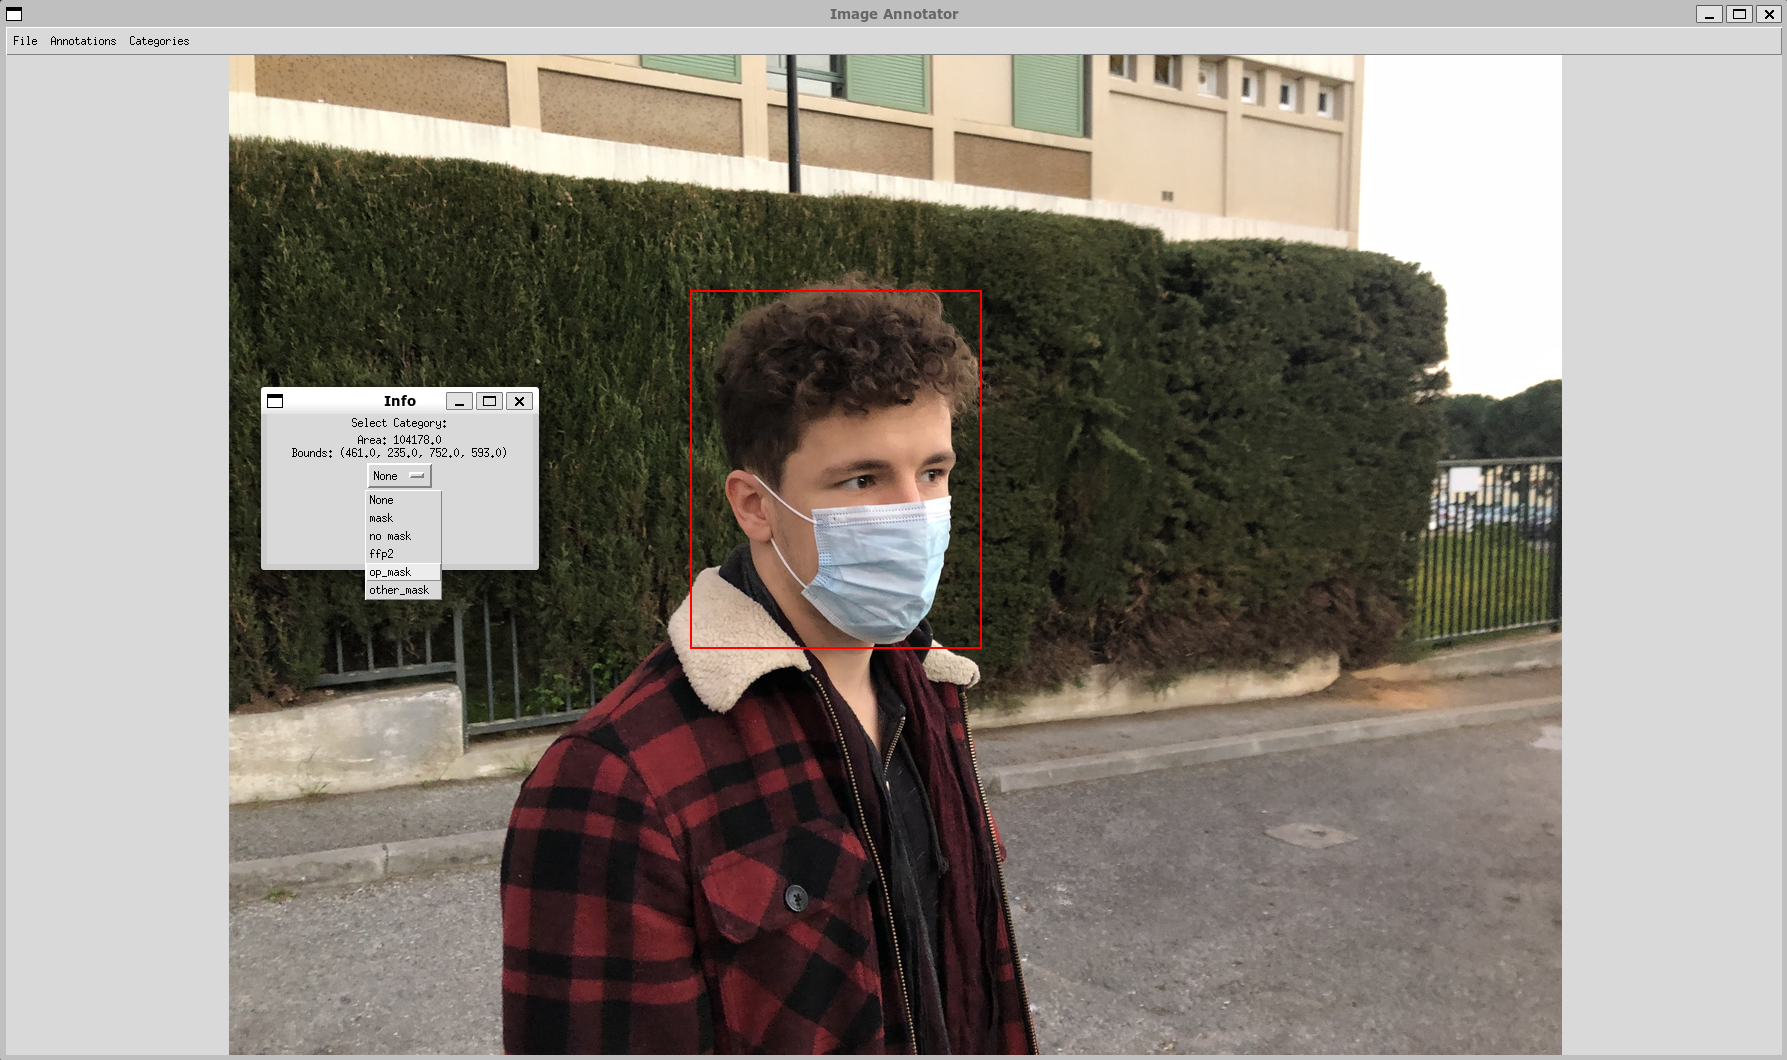
\includegraphics[width=\textwidth]{annotator_in_action.png}
    \caption{image annotator in action}
    \label{fig:anno}
\end{figure*}
\lstinputlisting[language=json,firstnumber=1,breaklines,caption={reduced example of saved annotations},captionpos=b, numbers=right]{../code/annotations.json}
The helping features are implemented as functions, that can be called through
the given menus:

\begin{description}[font=\sffamily\bfseries, leftmargin=1cm, style=nextline]
    \item[open image]
        Opens a file selector to let you chose an image to annotate
    \item[load next image]
        Finds the next image after natural order (the windows file-name order) in
        the same folder as the currently loaded image
    \item[save/import/view annotations]
        Lets the user chose a file location to either import or export all
        annotations as well as gives the possibility of viewing all currently
        loaded annotations in a list-view
    \item[add/replace/show category]
         Lets the user add a new category, replace an existing one or show all
         current categories in a list
    \item[import/export categories]
        Similar to annotations this gives the possibility to only share the
        categories by enabling exporting to json, csv or xlsx and importing from
        json and csv
    \item[replace/change destination]
        A feature that was not used during this project enabling the user to
        save each image resized and as png but not cropped to a specified
        location, that can be different for each image
\end{description}

Finally the main features of the annotation lay all in event listeners for the
mouse pointer. The user is able to draw rectangles in case an image was loaded.
A rectangle is only allowed if it has an area greater that 40 pixels, sides
longer than 5 pixels and is not overlapping with another rectangle by more than
20\%. Is a valid rectangle drawn, the user gets pointed details and is able to
chose a label. Figure \ref{fig:anno} shows the annotator in action. By
double-clicking or right-clicking the rectangle, this popup can be shown again
at any time and the label changed. Right-clicking also gives the choice of
deleting the rectangle.
\newline
This gives the annotator the full needed functionality and enables a quick and
easy labeling of all the images. Once the labeling is done, the menu item
"\textbf{crop and save}" reloads each image at a time, crops all made rectangles
to 240x240 square format and saves them in folders according to their labeling
in an by the user specified location.

\subsection{Machine Learning Model}

The Classifier is coded in python as well using the tensorflow library,
specifically the keras API, which is one of the most used deep learning
frameworks. In addition the OpenCV library is used again for face recognition. 
\newline
The overall structure on this part of the project is based on the tensorflow
tutorials \cite{tut}. It is split up into loading and structuring the dataset,
pre-processing the images, then training the model and finally evaluating it's
effectiveness. In addition to that the code offers interfaces for using the
model to classify any kind of image, or even live-feed through a camera.
\newline
The first part into any machine learning algorithm is the dataset. This is used,
to first train the network, by giving it an image to predict and based on the
answer improving its decision process through backpropagation. After complete
training, or even while the training process the dataset can also be used to
determine the accuracy of the prediction. In order for this evaluation not to be
biased, the dataset has to be split into a train and a test or validation set:
\lstinputlisting[
    language=json,
    breaklines,
    caption={splitting the dataset},
    captionpos=b
    ]{../code/dataset.py}
This way the training can be done on separate data than the final validation of
the effectiveness of the model. Otherwise it could be, that the model can
specifically classify the images it trained on, but nothing else.
\newline
Next come the pre-processing. Especially with smaller datasets like the one used
here, it makes sense to gain a little more data by augmenting the images and
creating multiple different ones from one. This is done by random rotations,
shifts, flips and sometimes even change of contrast or similar features (Listing
3, line 1-9). The code used here was supported by the examples on the keras
documentation page \cite{imageDataGenerator}.
\newline
A ML model has also problems with non-binary categorizations, which is why so
called one hot encoding on the labels can be helpful or even necessary (Listing
3, line 11,12). 
\newline
A common pre-processing step with images, is also the rescaling of color-values.
Usually they are saved as integer from 0 to 255. For a neural network it can be
easier to work with values between 0 and 1, which is why they can be rescaled by
multiplying each value with 1/255 (Listing 3, line 2).

\lstinputlisting[
    language=json,
    firstnumber=1,
    breaklines,
    caption={data augmentation and one hot encoding},
    captionpos=b
    ]{../code/preprocessing.py}

Now finally it is time for the model creation, compilation and training or
fitting. In the keras framework it is pretty simple to set up the layers one
wants to use in the network by simply adding them in order to the model. This
step is crucial, as it creates the overall network structure and determines how
good the model can be trained later. 
\newline
The model was inspired by multiple sources and refined by trial and error
\cite{Prakash2020}. \lstinputlisting[ language=json, firstnumber=1, breaklines,
caption={model layer structure}, captionpos=b, numbers=right ]{../code/model.py}
It uses alternating layers of convolution and max-pooling. This is the general
approach taken when doing an image classification. The convolution-layer uses a
filter to highlight certain features in the image, like edges for example, while
the max-pooling layers are responsible for summarizing pixels and therefore
simplifying the process. When going through training, the neural network will
adjust the filters used in the convolution-layers. Each convolution-layer has
the option relu (Rectified Linear Unit), which takes care, that all negative
values are turned into positive ones, so that the network doesn't get confused.
At the bottom there eventually is a flattening-layer as well as two
dense-layers. As the convolution-layers work with image-data, represented as
matrixes; they need to be flattened back to one dimension in order for the
network to make a decision. Finally the two dense-layers are condensing the
output down to exactly the number of classes we have so that the network is able
to gives us an answer. Before the the dense-layers we also added a
dropout-layer, that will already eliminate low confidences, so they won't mess
up any other information reaching that state.
\newline
After setting up the structure, the model can be compiled using an optimizer as
well as what should be optimized and finally fitted to the dataset. Especially
while the fitting process it is important to specify a good amount of training
epochs the model should go through, as using to few will leave potential unused
and using to many will take a lot of time, and not do any more good.
\lstinputlisting[
    language=json,
    firstnumber=1,
    breaklines,
    caption={model compilation and fitting},
    captionpos=b, 
    numbers=right
    ]{../code/compile_and_fit.py}
The loss-function we used, is the "mean\_squared\_error"-function as it performed
slightly better compared to the other loss-functions. More details on that
follow in the next chapter.
\newline
Some problems came up during development. 
\newline
To make the model easier accessible, the functionality was added to the image
annotation software as well. It offers a new tab in the top menu bar with a few
functions:
\begin{description}[font=\sffamily\bfseries, leftmargin=1cm, style=nextline]
    \item[auto detect faces]
        uses the OpenCV haarcascades, as explained before, to detect all faces
        on the image and automatically places the boxes in the annotator; the
        label is per default "None" ready for classification
    \item[train model]
        this lets the user chose a directory which includes all labeled folders
        with the respective dataset images; using this directory it loads the
        dataset and trains the model; the output window unfortunately only shows
        the whole output in the end, so the user has to wait a while
    \item[save/load model]
        saves or loads the model in two separate files; one contains all keras
        settings needed to run the model, the other one, contains label names as
        well as necessary images sizes for the model to integrate into the
        annotator 
    \item[classify current image]
        this function takes all boxes drawn on the current window, that where
        labeled with "None", crops them, and lets the model decide the correct
        label; the label is set automatically and displayed on screen together
        with all confidences
    \item[live classification]
        this is an experimental feature, that opens the camera and for each
        shown frame, uses the OpenCV library to cut out faces and plugging them
        into the ML model; in the end it is able to tell on the live feed
        whether a person is wearing a mask or not
\end{description}


\section{Testing and Results}

\section{Summary and Outlook}

In this project the entire process from creating a dataset until training and
using a neural network were shown. Even though the dataset was very small and
not professionally created, the produced neural network is able to detect many
different faces and can accurately determine wether a person is wearing no mask,
an op-mask or a ffp2-mask.
\newline
The provided tests show promising results, but of course there is still room for
improvement. Mentioned multiple times now, recreating the dataset would be the
first step in this direction. Especially if a goal would be for the program to
recognize any human on earth, there is a lot of training data missing. Right now
the program is most likely racist in a lot of different ways, as from it's
training data it is only used to the faces of the team members.
\newline
Another obvious step for the future would be running a proper tuner on the model
to better determine a lot of the hyperparameters. This includes mostly the
specific layer settings. Fine tuning the model can probably get the accuracy to
values consistently over 90%.
\newline
This project has nicely shown, how accessible the technology of machine learning
is nowadays and how easy it can be to implement an already very powerful model.
In our opinion machine learning and the development of "artificial intelligence"
will play a big role in the future. It has a lot of still unused potential.
With how easy it is to get started in the topic, building up a basic knowledge
in this area is recommended for every software engineer and even hobbyist.
\newline
We are very much looking forward to further experimentation and learning in
machine learning.

%%%%%%%%%%%%%%%%%%%%%%%%%%%%%%%%%%%%%%%%%%%%%%%%%%%%%%%%%%%%%%%%%%%%%%%%%%
% 	Acknowledgements
%%%%%%%%%%%%%%%%%%%%%%%%%%%%%%%%%%%%%%%%%%%%%%%%%%%%%%%%%%%%%%%%%%%%%%%%%%

%\section*{Acknowledgment}
%\addcontentsline{toc}{section}{Acknowledgment}

%%%%%%%%%%%%%%%%%%%%%%%%%%%%%%%%%%%%%%%%%%%%%%%%%%%%%%%%%%%%%%%%%%%%%%%%%%
% 	References
%%%%%%%%%%%%%%%%%%%%%%%%%%%%%%%%%%%%%%%%%%%%%%%%%%%%%%%%%%%%%%%%%%%%%%%%%%

% trigger a \newpage just before the given reference
% number - used to balance the columns on the last page
% adjust value as needed - may need to be readjusted if
% the document is modified later
%\IEEEtriggeratref{8}
% The "triggered" command can be changed if desired:
%\IEEEtriggercmd{\enlargethispage{-5in}}

% references section
% NOTE: BibTeX documentation can be easily obtained at:
% http://www.ctan.org/tex-archive/biblio/bibtex/contrib/doc/

% can use a bibliography generated by BibTeX as a .bbl file
% standard IEEE bibliography style from:
% http://www.ctan.org/tex-archive/macros/latex/contrib/supported/IEEEtran/bibtex
%\bibliographystyle{bibliography/IEEEtran}
% argument is your BibTeX string definitions and bibliography database(s)
%\bibliography{bibliography/IEEEabrv.bib,bibliography/references.bib}
%
% <OR> manually copy in the resultant .bbl file
% set second argument of \begin to the number of references
% (used to reserve space for the reference number labels box)
%\begin{thebibliography}{1}
%
%\bibitem{ref:kopka}
%H.~Kopka and P.~W. Daly, \emph{A Guide to {\LaTeX}}, 3rd~ed.\hskip 1em plus
%  0.5em minus 0.4em\relax Harlow, England: Addison-Wesley, 1999.
%
%\end{thebibliography}

%%%%%%%%%%%%%%%%%%%%%%%%%%%%%%%%%%%%%%%%%%%%%%%%%%%%%%%%%%%%%%%%%%%%%%%%%%
% 	End of the document
%%%%%%%%%%%%%%%%%%%%%%%%%%%%%%%%%%%%%%%%%%%%%%%%%%%%%%%%%%%%%%%%%%%%%%%%%%

\end{document}


